\subsection{Caso d'uso UC10: Creazione dell'infografica}
\begin{figure}[h] 
	\centering 
	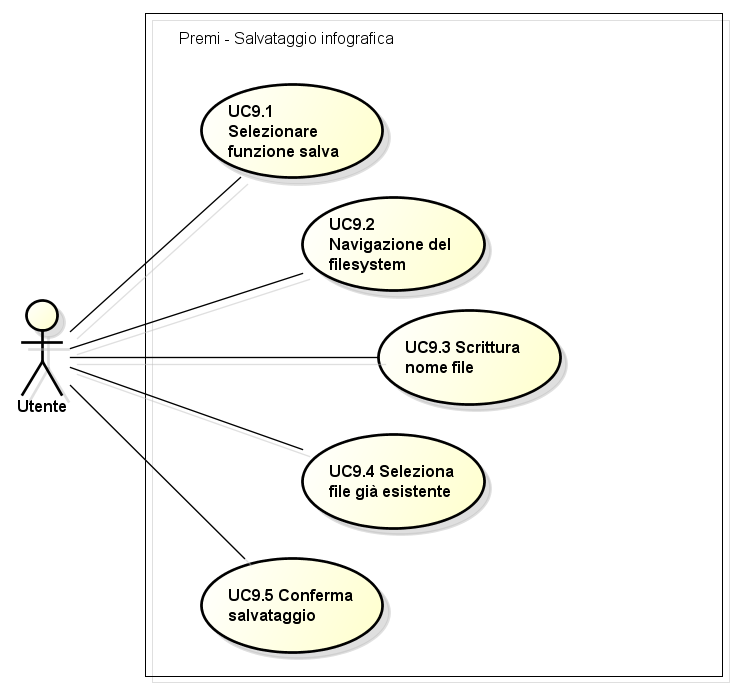
\includegraphics[scale=0.45] {img/UC10.png} 
	\caption{UC10 - Creazione dell'infografica} 
\end{figure}

\begin{itemize}
	\item \textbf{Attori:} Proprietario;
	\item \textbf{Scopo e descrizione:} L'utente ha creato una presentazione e da questa vuole creare un'infografica. Con l'opportuno tool, può scegliere il template da usare e le slide da includere in essa. Una volta completata la procedura verrà creata l'infografica corrispondente;
	\item \textbf{Precondizione:} L'utente ha creato una presentazione e ha selezionato il comando per creare l'infografica;
	
	\item \textbf{Flusso principale degli eventi:}
	\begin{enumerate}
		\item L'utente sceglie un template [UC10.1];
		\item L'utente sceglie le slide da inserire nell'infografica [UC10.2];
		\item L'utente conferma la creazione dell'infografica [UC10.3];
	\end{enumerate}
	\item \textbf{Postcondizione:} Il sistema ha creato l'infografica a seconda delle scelte dell'utente.
\end{itemize}


\subsection{Caso d'uso UC10.1: Scegliere un template}
\begin{itemize}
	\item \textbf{Attori:} Proprietario;
	\item \textbf{Scopo e descrizione:} L'utente sceglie il template con cui creare l'infografica;
	\item \textbf{Precondizione:} Il sistema ha aperto la finestra di dialogo per la scelta del template;
	\item \textbf{Postcondizione:} Il sistema registra la scelta del template fatta dall'utente.
\end{itemize}


\subsection{Caso d'uso UC10.2: Scegliere le slide}
\begin{itemize}
\item \textbf{Attori:} Proprietario;
\item \textbf{Scopo e descrizione:} L'utente sceglie quali slide del suo progetto inserire nell'infografica;
\item \textbf{Precondizione:} L'utente ha scelto il template con cui creare l'infografica;
\item \textbf{Postcondizione:} Il sistema registra la scelta delle slide fatta dall'utente.
\end{itemize}


\subsection{Caso d'uso UC10.3: Conferma della creazione dell'infografica}
\begin{itemize}
\item \textbf{Attori:} Proprietario;
\item \textbf{Scopo e descrizione:} L'utente vuole confermare la creazione dell'infografica;
\item \textbf{Precondizione:} L'utente ha scelto il template e le slide con cui creare l'infografica;
\item \textbf{Postcondizione:} Il sistema ha creato l'infografica.
\end{itemize}